\Chapter{Tervezés, implementáció}

\Section{A WebGL-ről}
A WebGL, azaz Web Graphics Library, egy 2D és 3D grafikus renderelésre képes JavaScript alapú API, amely lehetőséget ad interaktív grafika megjelenítésére a webböngészőkben, bármilyen más harmadik féltől származó bővítmény használata nélkül. Képes teljes mértékben hasznát venni a hardveres gyorsításnak, a képfeldolgozási utasításokat a GPU-val hajtatja végre. 

Első verzióját 2011 március 3.-án adta ki a Khronos Group, azóta is ők fejlesztik. A Khronos Group emelett még sok más grafikai alkalmazásprogramozási felületet készít, melyek közül a két legismertebb talán az OpenGL és a Vulkan.

A WebGL az OpenGL ES-en alapszik, mely amint a nevéből is adódik, beágyazott rendszerekhez készült. Széles körben használatos főleg mobiltelefonok, tableteken, és más hordozható készülékeken. A WebGL első verziója az OpenGL ES 2.0-án alapult, azóta már kiadták a 2.0-ás verziót, amely az OpenGL ES 3.0-t vette alapul.

Az 1.0-ás verziót már szinte az összes modern webböngésző támogatja, valamint a HTML5 szabványnak is része. A 2.0-ás verziót még sok böngésző csak részlegesen támogatja, néhány pedig, mint például a Microsoft Edge, egyáltalán nem.

A WebGL API nagyon alacsony szintű természete miatt nem célszerű natívan programozni. Az alap alakzatok megjelenítése is rengeteg időt venne igénybe ilyen megvalósítással. Emiatt is készült rengeteg függvénykönyvtár hozzá, amelyek lényegesen megkönnyítik a fejlesztési folyamatot, magasszintű felületet biztosítanak egyszerű alakzatok megjelenítésére, textúra beolvasására, UV map előállításához, projekciós és modelview mátrixok kiszámolásához.

Az egyik ilyen híres függvénykönyvtár a Three.js. A Three.js nagyon bő funkcionalitással rendelkezik, egyszerűen létrehozható vele scene, renderer, kamera. Képes irányított és pontszerű fényforrások kezelésére. Megkönnyíti a materialok használatát, animációk létrehozását, és még sok más hasznos funkciót tartalmaz.

A Three.js-ben először is egy scene-t kell létrehoznunk, ebben az objektumban fog történni a kirajzolás. Ezután jön a renderer létrehozása, majd egy kamera objektum hozzáadása a scenehez. Ha ezek megvannak, a meglévő scenehez hozzá lehet adni a kívánt objektumokat, azaz fényforrásokat, irányítást megvalósító objektumokat, valamint mesheket. A mesheket a Three.js-ben lehetőség van JSON objektumokból betölteni, majd dinamikusan hozzájuk rendelni materialt. Az animate függvényben meghívva a renderer kirajzoló függvényét frissül a megjelenés.
\Section{Unity}
A Unity Engine egy, a Unity Technologies által fejlesztett játékmotor. Elsőként az Apple Worldwide Developers Conference nevű rendezvényén mutatták be 2005-ben. Célja kezdetektől a játékfejlesztés folyamatának megkönnyítése. Ennek érdekében az új fejlesztők számára könnyen tanulhatóvá alakították ki a működését, sok ''Drag and Drop'' funkció található benne. Másik szempontból viszont több platformra is egyszerű vele fejleszteni, mára már több mint 25 különböző platformot támogat, ezzel megkönnyítve a cross-platform alkalmazások fejlesztését. Maga a motor elsősorban bár játékmotornak lett kialakítva, de sok más területen is használják, beleértve a filmipart, autóipart, és az építőipart.

Kezdetben egy Boo nevű programozási nyelvet használt a különböző szkriptekhez, de ezt később felváltotta a JavaScripten alapuló UnityScript nevű nyelv. Mára viszont a UnityScriptnek is csak részleges támogatottsága van. Ez annyit tesz, hogy nem lehetséges többé ilyen szkripteket létrehozni a motor újabb verzióiban, de a régebbi projekteket amelyek ilyen típusú szkripteket tartalmaznak még tudja kezelni. A használatos nyelv helyette a C\#, melynek támogatottsága előreláthatólag a fejlesztők nyilatkozatai szerint a jövőben csak bővülni fog. Maga a motor futási időben C++ kódot futtat, ebbe ágyazódnak be wrapperekkel a más nyelven megírt szkriptek.

Licenszét tekintve a szoftvernek három kiadása van: az ingyenes Personal, és a fizetős Pro valamint Plus verziók.Ezek között sok különbség nincsen, a fizetős kiadások főbb újdonságait a fejlesztők által nyújtott plusz szolgáltatások teszik ki, mint például az online tárhely, vevőszolgálatnál előnyben részesülés, oktató tanfolyamok, stb. Viszont léteznek korlátozások az egyes kiadások felhasználására. Az ingyenes változatot csakis személyes használatra, vagy évi \$100,000 bevételt meg nem haladó üzleti célra lehet felhasználni. A Plus verziónál a megengedett bevételi korlát \$200,000, míg a Pro verzió korlátlanul használható.

Amint említettem sok platformot támogat, ezek közé tartozik a WebGL is. A továbbiakban ezen platform sajátosságait részletezném.
\subsection{Unity WebGL}
A WebGL magasabb szintű absztrakciós keretrendszerei közé tartozik néhány játékmotor is. Ezek közül a két legismertebb az Unreal Engine és a Unity Engine. Ezek WebGL-beli teljesítménye bár nem egyezik meg az olyan grafikus APIk-éval mint a Direct3D, Vulkan, vagy OpenGL, mégis egy jelentős megszorítást küszöböl ki azzal, hogy teljesen közvetlen hozzáférést biztosít a számítógép grafikus kártyájához.

Implementáció szempontjából nincs különbség a platformok között Unityben, a sajátosságok a fordításkor jönnek elő. WebGL build esetén a kimeneti fájlok közé tartozik egy HTML fájl amelybe be van ágyazva a WebGL applikáció, egy TemplateData mappa amely tartalmazza a weboldal és a lejátszó megjelenését leíró fájlokat, valamint egy Build mappa, amely tartalmazza a WebGL tartalom betöltéséhez szükséges JavaScript fájlokat, valamint a projekt által használt összetevőket, tömörített unityweb állományokban.

Mivel a WebGL csakis JavaScript kódot tud futtatni, a Unity pedig C\# szkripteket használ, futási időben pedig C++ kódot futtat, szükséges a build folyamán a kód átkonvertálása. Ez több lépésben történik, először is a .NET kódot egy IL2CPP, azaz Intermediate Language To C++ nevű technológiával átalakítja C++ forráskóddá.  Ha ez megtörtént, a létrejött C++ kód az Emscripten nevű compiler segítségével átfordul JavaScript kóddá. Az így létrejött forrás már futtatható egy weboldal WebGL lejátszójában.
\subsection{Unity Editor}
A program működésének kialakításában a szkripteken kívül a másik nagy szerepet az editor tölti be. Az editorból elérhető a projekthez hozzáadott összes erőforrás, azaz a textúrák, materialok, meshek, szkriptek, valamint az összes létrehozott scene.
Az editor beépítve tatalmazza a Unity Asset Store-t, ahonnan le lehet tölteni fizetős és ingyenes komponenseket, legyen az szkript, mesh, vagy bármilyen más építőelem. A projekthez innen szereztem be az autók, a buszok, az épületek, a fák, és a szökőkutak modelljét.

Az editorban egy scene megnyitása után megjelenik annak jelenlegi állapota. Ez azt jelenti, hogy kilistázza a benne elhelyezett GameObject objektumokat, valamint megjeleníti azokat a világban. A scene 3D-s megjelenítőjében szabadon mozgatható bármely objektum, egyet kiválasztva pedig megnyílik a rá vonatkozó inspector. Az inspector kilistázza a kiválasztott GameObject összes komponensét, valamint azoknak paramétereit. Ezeket a paramétereket innen meg lehet változtatni, melynek hatása egyből meg is jelenítődik. Az objektumoknak kötelezően lennie kell Transform komponensének, mely a világban lévő pozíciójukat írja le x, y, és z koordinátákkal, valamint szintén ezen három tengelyen való forgatásukat és skálázásukat.
Az inspectorban lehetséges hozzáadni objektumokhoz új komponenst, mely lehet beépített elem, vagy egy megírt C\# szkript. A scene-en belül lehetséges az objektumok között hierarchia kialakítása is, azaz egy objektum lehet más objektumoknak a szülője.
Az objektumokat el lehet látni tag-ekkel, melyek segítségével szkripteken belül egyszerűen beazonosíthatóvá válnak.
\begin{figure}[H]
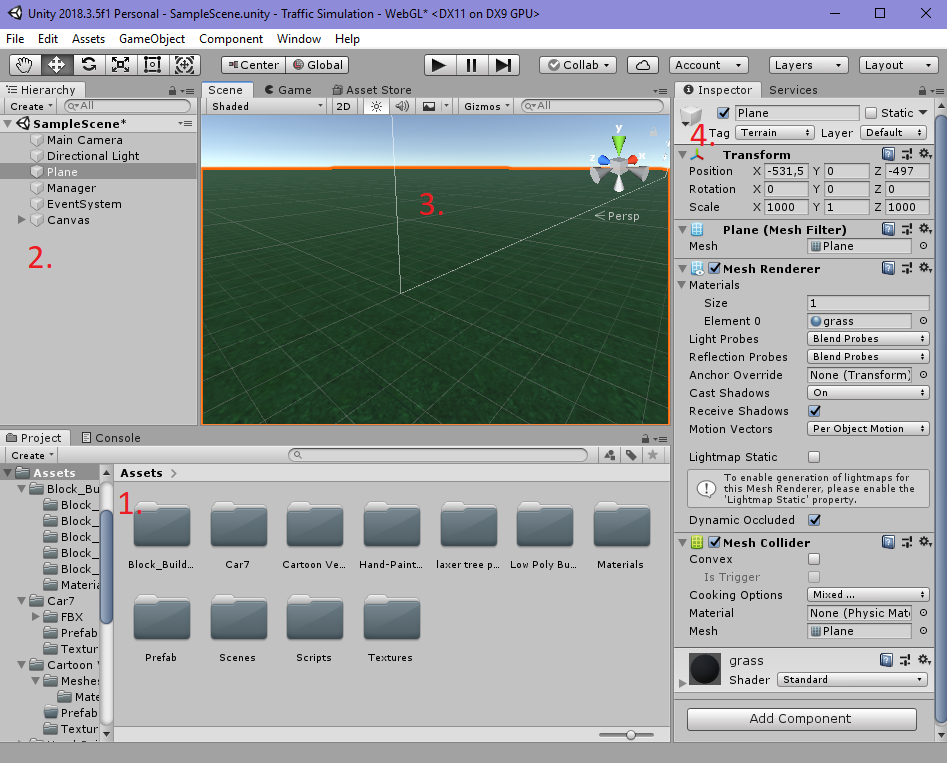
\includegraphics[width=\linewidth]{editor.png}
\caption{Az editor részei megszámozva: 1: Projekt erőforrásai 2: A Scene összes objektuma 3: A Scene objektumainak világon belüli reprezentációja 4: Inspector}
\label{fig:ed}
\end{figure}
A projekt erőforrásaihoz lehetséges hozzáadni sablon GameObject objektumokat is, azaz a scene-en belül létrehozott egyik objektum jelenlegi állapotát mentjük le, az összes komponensével, azoknak jelenlegi állapotaival együtt. Az így lementett erőforrás szkriptek segítségével dinamikusan hozzáadható a scene-hez futási időben. A szkripteken belüli publikus adattagok inicializálhatóak az editorból, az inspector segítségével. Ezen adattagok bármilyen típust felvehetnek, beleértve minden különböző típusú erőforrást.
Ezzel lehetséges referenciát átadni a szkripteknek egy adott GameObjectről, materialról, vagy bármilyen scene-en belüli objektum komponenséről.
\Section{Szimuláció tervezése}
A szimuláció felépítését tekintve a következők mondhatóak el. Először is felhasználja a már legenerált úthálózatot, azon a járművek mozgásának alapjaként szolgál egy véletlenszerű részgráf, amely a bejárandó útvonalat reprezentálja.
A járművek mozgásához felhasználom a Unity fizikai motorját, amely kvázi realisztikusan képes szimulálni a kerekek mozgásából, azok ívéből a jármű haladási irányát, sebességét, illetve a fékezés szimulálásához felhasználható eszközt nyújt, mellyel ténylegesen csak a kerekek forgásának sebességét csökkentem, ami közvetetten csökkenti a jármű sebességét.
\subsection{Szenzorok}
A járműveknek a környezettel és egymással való interakciója érdekében úgynevezett szenzorokat használok. Ez nem más, mint a fizikai motor egy raycast függvénye, mely egy pontból kiindulva a megadott irányvektornak megfelelő irányba, megadott hosszúságú sugarat bocsát ki. Ennek lehetséges lekérdezni az első, más objektum ütköző komponensével történt metszéspontját. Visszaadja valamint azt is, hogy ezen metszéspontnál melyik másik objektummal találkozik.
Az észlelt objektum meghatározására annak tag-jét használom fel.
A következő szabályokat alkalmaztam az esetek lekezelésére:
\begin{itemize}
\item{Ha egy jármű szenzora másik járművel találkozik, akkor a két jármű távolságának fordított arányában korlátozza a maximális sebességet.}
\item{Ha egy jármű szenzora útkereszteződést észlel, és a jármű kanyarodni fog, vagy pedig kanyar következik, akkor maximális sebességét korlátozza az eredeti harmadára.}
\item{Ha egy jármű szenzora olyan buszmegállót észlel, amiben éppen busz tartózkodik, álljon meg és engedje el a buszt.}
\item{Ha egy jármű szenzora olyan útkereszteződést észlel, ahol az ő oldaláról éppen piros a jelzőlámpa, akkor álljon meg.}
\item{Ha egy jármű szenzora választóvonalat észlel a jármű bal szélétől jobbra, és a jármű nincsen éppen útkereszteződésben, akkor kanyarodjon enyhén jobbra.}
\item{Ha egy jármű szenzora többsávos út sávelválasztóját észleli a jármű bal szélétől jobbra, és a jármű nincs éppen útkereszteződésben, és a következő lehetőségnél jobbra fog fordulni, akkor enyhén kanyarodjon jobbra.}
\end{itemize}
\subsection{Szükséges objektumok}
A szimulációban résztvevő járművek példányosításához létrehoztam néhány sablon objektumot, azaz prefab-et. Ezek a személygépjármű és az autóbusz objektumok.
Az alap objektumokat a Unity Asset Store-ból szereztem be, ezek alapjában véve tartalmazták a mesht, egyesével elkülönítve a négy kereket. Az alap objektum felépítése a következő képpen néz ki:
Van egy főobjektum, mely gyerekelemként tartalmazza a karosszéria mesh-ét, valamint egy Wheels objektumot. Ez a Wheels objektum rendelkezik négy gyerekelemmel, melyek rendszerint a négy keréknek felelnek meg.
A busz és az autó felépítése ilyen szempontból megegyezik, a hozzáadott komponensek is megegyezőek lesznek. A kettő közötti különbséget a hozzárendelt szkript fogja majd adni.
\subsubsection{Komponensek hozzáadása}
Kezdésként a főobjektumhoz hozzáadtam egy Rigidbody komponenst. Ezen komponens által lehet befolyásolni az objektum működését a fizikai motoron belül, szükséges az ütközések vizsgálatához is. Ezen Rigidbody komponensen belül beállítottam az autó tömegét 1200 egységre, a buszét pedig 1400 egységre.

Következő lépésben szükséges a járművek kerekeihez WheelCollider komponenseket rendelni. Ezen komponens számolja ki a fizikai motoron keresztül a kerekek fordulatszámát, csúszását, ennek a komponensnek a manipulálásával lehet gázt és féket, valamint a kormányzást szimulálni. A szkriptben szükség lesz erre a komponensre való hivatkozásra, ezért nem a meglévő kerekekhez adom hozzá, hanem létrehozok a kerék objektumokból egy másolatot.
Ezekből a másolatokból törlök minden komponenst, és hozzáadok egy WheelCollidert. Ennek a sugarát beállítom a megfelelő mértékre mindkét járműnél, hogy lefedje a kerék meshét. Az így létrehozott objektum hivatkozható a szkriptben anélkül, hogy egy teljes GameObject-et kéne hozzárendelni, mivel ezek az objektumok csak egyetlen komponensből állnak a Transformon kívül.

A főobjektumba elhelyeztem rendszerint egy CarEngine és egy BusEngine szkriptet. A BusEngine a CarEngine leszármazottja, minimális módon fog eltérni az autó szkriptjétől.
Végül a karosszériát reprezentáló objektumhoz hozzáadtam egy mesh collider komponenst, mely az ütközések vizsgálatára, a szenzorok működéséhez szükséges.
\subsection{Szimulációs szkriptek}
\begin{figure}[H]
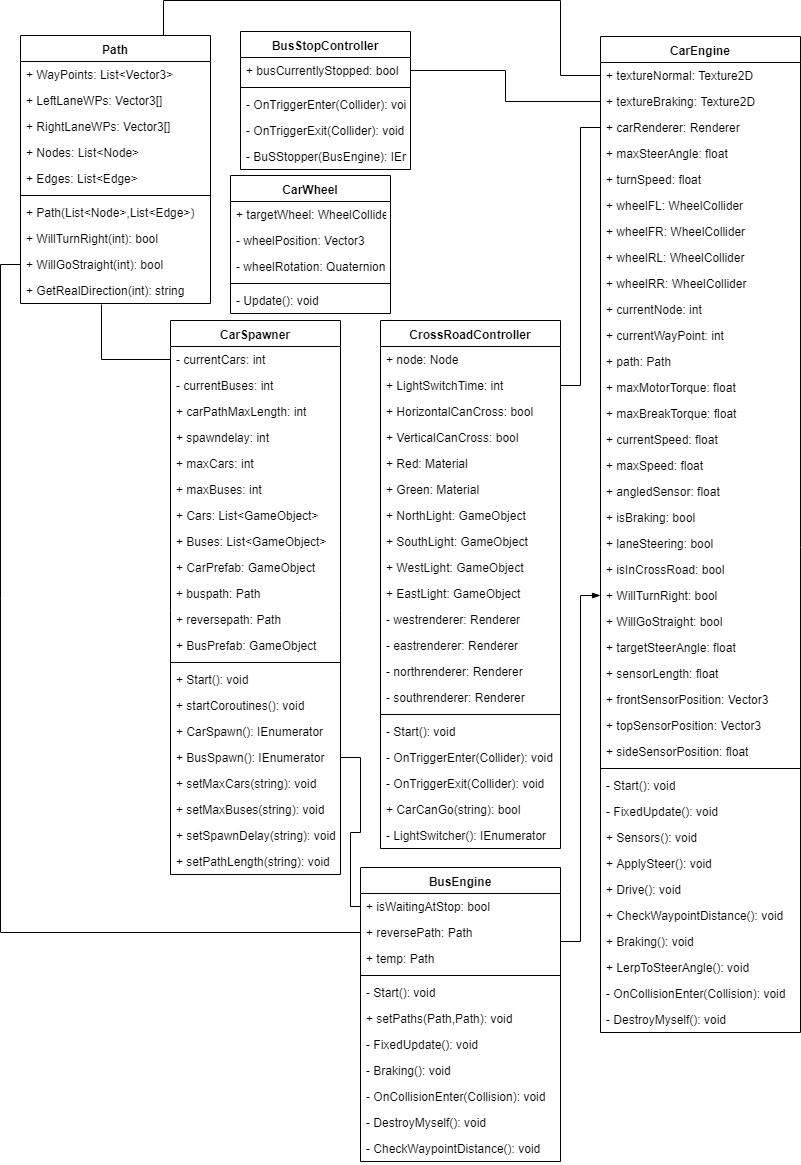
\includegraphics[scale=0.53,keepaspectratio]{simuml.png}
\caption{A szimulációval foglalkozó szkriptek UML osztálydiagramja}
\label{fig:simuml}
\end{figure}
\subsubsection{Path}
Ez az osztály adja vissza a járműveknek az egyedi útvonalaikat. Adattagjai közé tartozik egy WayPoints nevű Vector3 lista, amely a célpontok koordinátáinak a listája, egy LeftLaneWPs és egy RightLaneWPs Vector3 tömb, amelyek a többsávos utak esetén tárolják a két a belső és külső sávra vonatkozó célpontokat. Tartalmaz továbbrá egy Node és egy Edge típusú listát, amely a gráf csomópontjait és éleit tartalmazza.

Két csomópont között a haladási irány kiszámítására írtam egy GetRealDirection függvényt. Ez a függvény paraméterként megkapja a következő csomópont indexét, ami hogyha megegyezik a jelenlegi él célpontjával, akkor visszaadja az él haladási irányát, ellenkező esetben annak ellentetjét adja vissza.
\begin{cpp}
public string GetRealDirection(int idx)
        {
            if(Nodes[idx] == Edges[idx].To)
            {
                return Edges[idx].Direction;
            }
            else
            {
                switch (Edges[idx].Direction)
                {
                    case "north":
                        return "south";
                    case "south":
                        return "north";
                    case "west":
                        return "east";
                    case "east":
                        return "west";
                    default:
                        return null;
                }
            }
        }
\end{cpp}

Szintén írtam két függvényt annak meghatározására, hogy egy adott csomópont elérése után a jármű jobbra fog-e kanyarodni, illetve egyenesen megy-e tovább. Ezek a WillTurnRight és a WillGoStraight metódusok. Ezek működésükben a GetRealDirection metódust használják fel a jelenlegi és a következő csomópontra, majd a kettő kapott értéket vizsgálva meghatározzák hogy kanyarodik-e, illetve egyenes megy-e tovább.
\begin{cpp}
public bool WillTurnRight(int idx)
        {
            if(idx < Nodes.Count - 2)
            {
                string currentlyGoing = GetRealDirection(idx);
                string willGo = GetRealDirection(idx + 1);
                if ((currentlyGoing == "north" && willGo == "east") || 
                (currentlyGoing == "east" && willGo == "south") ||
                (currentlyGoing == "south" && willGo == "west") || 
	     (currentlyGoing == "west" && willGo == "north"))
                {
                    return true;
                }
            }
            
            return false;
        }
\end{cpp}
A másik metódus működésében megegyezik a fentivel, azzal különbséggel hogy a két érték egyenlőségének esetén ad igaz értéket, ellenkező esetben hamisat.

Az útvonalat a konstruktor adja vissza, mely megkapja az érintett csomópontok és élek listáját. Először is megnézi hogy a kapott út tartalmaz-e éleket, vagy pedig csak egy pontból áll. Ha valós útvonal, akkor a kijelöli a kezdőpontot az első él irányának függvényében. Példaként ha dél felé tart az él, akkor a kezdőpont az első csomópont középpontja és bal felső csúcsa közötti felezőpont. Ha az él iránya dél felé tart, de kiindulási pontja a következő csomópont, akkor a kezdőpont a csomópont középpontja és jobb alsó csúcsa közötti felezőpont lesz.
\begin{cpp}
case "south":
    if (nodes[1] == edges[0].From)
    {
        WayPoints[0] = (nodes[0].WorldCornerBR + 
        WayPoints[0]) / 2;
    }
    else
    {
        WayPoints[0] = (nodes[0].WorldCornerTL +
         WayPoints[0]) / 2;
    }
    break;
\end{cpp}
Ezek után végigiterál az útvonal további pontjain, ezzel megegyező módszerrel kiszámolja a célpontokat. Ha egy adott élen a sávok száma 2, akkor kiszámolja a RightLaneWPs és LeftLaneWPs adott indexű elemeit, majd a haladási iránynak megfelelően cseréli az adott célpontot a következő módon:
\begin{cpp}
if (edges[i - 1].Lanes == 2)
{
    LeftLaneWPs[i] = (point + 
    WayPoints[WayPoints.Count - 1]) / 2;
    RightLaneWPs[i] = (nodes[i].
    WorldCornerBR + WayPoints[WayPoints.Count - 1]) / 2;
}
if (WillTurnRight(i-1))
{
    if(edges[i - 1].Lanes == 2)
    {
        WayPoints[WayPoints.Count - 1] = RightLaneWPs[i];
    }
    point = (nodes[i].WorldCornerBR + nodes[i].
    WorldCornerTR) / 2;
    WayPoints.Add((nodes[i].WorldCornerBR + point) / 2);
}
else if(!WillGoStraight(i-1))
{
    if (edges[i - 1].Lanes == 2)
    {
    WayPoints[WayPoints.Count - 1] = LeftLaneWPs[i];
    }
    point = (nodes[i].WorldCornerBL + nodes[i].
    WorldCornerTL) / 2;
    WayPoints.Add((nodes[i].WorldCornerTL + point) / 2);
}
else if(edges[i - 1].Lanes == 2)
{
    WayPoints[WayPoints.Count - 1] = LeftLaneWPs[i];
}
\end{cpp}

A konstruktor lefutása után az osztály WayPoints adattagja már tartalmazza az útvonal bejárásához szükséges összes pontot.
\subsubsection{CarSpawner}
Ez a szkript felelős a buszok és az autók létrehozásáért. Tartalmazza a következő publikus adattagokat, amelyeket a felhasználói felületről futás közben lehet módosítani:
\begin{itemize}
\item{carPathMaxLength: Egy autó útjának maximális hossza, csomópontokban mérve.}
\item{spawndelay: Két autó létrehozása közötti időtartam.}
\item{maxCars: Az egyszerre maximálisan létezhető autók száma.}
\item{maxBuses: Az egyszerre maximálisan létezhető buszok száma.}
\end{itemize}

Szüksége van magára a busz és autó objektumokra, ezek GameObject típusúak és az editorból rendelem hozzá őket. Az éppen létező autókat és buszokat külön GameObject típusú listában tartja nyilván.
Működése kettő korutinon alapszik, az egyik az autókat, a másik a buszokat hozza létre.
\begin{cpp}
IEnumerator CarSpawn()
{
    while (true)
    {
        yield return new WaitForSeconds(spawndelay);
        if(currentCars < maxCars)
        {
            Cars.Add(Instantiate(CarPrefab));
            Debug.Log("car created");
            Cars.Last().GetComponent<CarEngine>().path = 
            gameObject.GetComponent<RoadGenerator>().graph.
            GenerateRandomPath(carPathMaxLength);
            currentCars++;
        }
        for (int i = 0; i < Cars.Count; i++)
        {
            if (Cars[i] == null)
            {
                Cars.Remove(Cars[i]);
                currentCars--;
            }
        }
     }           
}
\end{cpp}
A korutinokat IEnumerator típusú függvényekként kell létrehozni. Ezen korutinok indulásuk után külön szálon futnak. Sajátosságok még az, hogy lehet őket várakoztatni, amelyre a ``yield return new WaitForSeconds()'' szintaktika ad lehetőséget.
A fenti korutin az autók létrehozásáért felelős. Egy végtelen ciklust futtat, melynek minden iterációja elején vár a spawndelay-ben megadott ideig. Ezután, ha kevesebb autó van eddig mint a megengedett, akkor hozzáad egy újat a listához, majd a létrejött autó CarEngine szkript komponensében beállítja az útvonalat, melyet RoadGenerator komponens gráfja fog generálni, hossza pedig függ a megadott változótól.

Mivel az autók céljuk elérésekor törlik magukat, a listából is el kell távolítani. Ez egy egyszerű null check, végigiterál a Cars listán és törli a null referenciájú elemeket.
A korutinok elindítása egy függvényben történik, mely a komponens betöltődésekor a Start-ban hívódik:
\begin{cpp}
public void startCoroutines()
        {
            StartCoroutine(CarSpawn());
            StartCoroutine(BusSpawn());
        }
\end{cpp}
A buszokért felelős korutin nagymértékben megegyezik az autókéval, annyi különbséggel hogy fix 10 másodperces késleltetés van, valamint azonos busz útvonalat kap mindegyik.
Ezt a szkriptet a Manager objektum komponenseként adom hozzá a scenehez.
\subsubsection{CarEngine}
A CarEngine szkript felel az autók összes mozgásáért. Az editorban inicializált adattagjai a következőek:
\begin{itemize}
\item{TextureNormal: Alap állapotban a jármű textúrája.}
\item{TextureBraking: Fékezés közben a jármű textúrája.}
\item{Négy WheelCollider objektum.}
\item{carRenderer: Az autó meshrenderer komponense.}
\end{itemize}
Az osztályon belül nyilván van tartva annak maximális kormányzási íve, maximális kanyarodási sebessége, a bejárandó út, az út hanyadik csomópontjánál jár, az úton hanyadik kijelölt célpontnál tart, a motor maximális forgatónyomatéka, a fék maximális ereje, a jármű jelenlegi sebessége, a jármű maximális sebessége, az hogy a jármű jelenleg fékez-e, sávot vált-e, útkereszteződésben van-e, jobbra fog-e kanyarodni, egyenesen fog-e menni, valamint a jelenlegi kormányzás íve.
Definiálva van továbbá a szenzorok pozíciója, ezek a jármű elején vannak bal oldalt, középen és jobb oldalt, valamint a jármű fölött szintén ugyan ilyen elrendezésben, hozzátéve még egyet, amelyik a járműtől jobbra néz.

A szkript start metódusa a következő:
\begin{cpp}
private void Start()
    {
        transform.position = path.WayPoints[0];
        if(path.WayPoints.Count > 1)
        {
            transform?.LookAt(path.WayPoints[1]);
        }
    }
\end{cpp}
Beállítja a jármű pozícióját az első célpontra, és ha az út nem csak egyetlen csomópontból áll (azaz tényleges útvonal), elforgatja a járműt a következő célpontja felé.
Az objektum animálására az Update metódus helyett a FixedUpdate-et használom. Ez azért előnyös, mert a fizikai számítások amelyek a képkockaszámtól függenek, a sima Update metódusban helytelenül működnének. A FixedUpdate ezzel a fizikai motor frekvenciáját használja. A metódus az alábbiakat tartalmazza:
\begin{cpp}
private void FixedUpdate()
    {
        Sensors();
        ApplySteer();
        Drive();
        CheckWaypointDistance();
        Braking();
        LerpToSteerAngle();
    }
\end{cpp}
Ebből az első, a Sensors metódus a szenzorokkal kapcsolatos számításokat végzi el. Megnézi ütközött-e valamelyik valamilyen objektummal, ha igen akkor elvégzi a hozzá tartozó műveleteket. Egy példa a sávelválasztó észlelésére:
\begin{cpp}
if (Physics.Raycast(sensorStartPos, Quaternion.AngleAxis(-angledSensor,
	 transform.up) * transform.forward, out hit, 3))
        {
            if (hit.collider.CompareTag("MultiLaneDivider") && 
            !WillTurnRight)
            {
                if (!isInCrossRoad)
                {
                    Debug.DrawLine(sensorStartPos, hit.point);
                    targetSteerAngle = -5f;
                    laneSteering = true;
                }

            }
        }
\end{cpp}
A metódus ezen része az autó bal oldala felé vetít sugarat, melynek hossza 3 egység. A sensorStartPos egy előre beállított vektor a szenzorok számára, a középső első szenzor helyét jelenti, a többi ehhez képest relatívan helyezkedik el. A második paraméter az y tengely körüli forgatást jelenti -90 fokkal (az angledSensor értéke). Ha a sugár ütközött, akkor az első feltétel teljesül, eltárolódik a hit változóba az érintett ütköző. A következő lépésben az érintett objektum tag-jét vizsgálom. Ha megegyezik a sávelválasztó tag-jével, valamint az autó nem akar jobbra kanyarodni, és nincs is útkereszteződésben, akkor balra 5 fokban kezd el kormányozni, és a sávváltást jelző változó igazra vált. Ez a változó a Sensors metódus elején mindig hamis értéket kap.

A következő metódus, az ApplySteer az amelyik kiszámolja hogy az autónak milyen irányba és mennyit kell kormányoznia. Ha az autó éppen sávot vált és nincs útkereszteződésben, a metódus nem csinál semmit. Ha ezek nem teljesülnek, megkapja a következő célponthoz tartó relatív vektort, amelynek hossza alapján kiszámolja a kormányzás kívánt szögét a következő képpen:
\begin{cpp}
Vector3 relativeVector = transform.InverseTransformPoint(path.
WayPoints[currentWayPoint]);
float newSteer = (relativeVector.x / relativeVector.magnitude)*
maxSteerAngle;
targetSteerAngle = newSteer;
\end{cpp}

A következő metódus a Drive, amely a jármű kerekeinek forgatásáért, valamint a fékezésért felelős. Első lépésben kiszámolja a jelenlegi sebességet a kerék kerületének és forgásának függvényében. Ezután ha gyorsabban megy, mint a maximális sebesség akkor fékez, ha lassabban akkor gázt ad, egyébként pedig nem ad gázt, és nem fékez.
\begin{cpp}
public void Drive()
    {
        currentSpeed = 2 * Mathf.PI * wheelFL.radius *
        wheelFL.rpm * 60 / 1000;
        if(currentSpeed < maxSpeed)
        {
            isBraking = false;
            wheelFL.motorTorque = maxMotorTorque;
            wheelFR.motorTorque = maxMotorTorque;
        }
        else if(currentSpeed > maxSpeed)
        {
            wheelFL.motorTorque = 0;
            wheelFR.motorTorque = 0;
            isBraking = true;
        }
        else
        {
            isBraking = false;
            wheelFL.motorTorque = 0;
            wheelFR.motorTorque = 0;
        }
        
    }
\end{cpp}

A következő metódus megnézi a jármű távolságát a következő célpontjától. Ezt a beépített Vector3.Distance függvénnyel teszi. Ha 2.5 egységnyi távolságon belülre ért, akkor megnézi ez-e az utolsó célpont, ha igen akkor törli saját magát. Ellenkező esetben, ha nem az utolsó előtti csomópontnál jár, akkor kiszámítja hogy a következő csomópontnál milyen irányba fog tovább menni. Ezt a Path osztály függvényeivel teszi. Ezek után inkrementálja a currentWayPoint változót, mely a soron következő célpont indexét jelöli. Ha nincs útkereszteződésben a célpont elérésekor, akkor a csomópontok indexét is növeli.

Fontos elkülöníteni itt a csomópont és a célpont fogalmát. Ahogyan az a modellben is definiálva lett, a csomópont az úthálózat szakaszainak összekötő részét jelöli, ami akár lehet útkereszteződés. A célpontok viszont a járművek részére kijelölt útvonal fix pontjai, amelyek egyértelműen kijelölik hogy az út melyik részén kell haladniuk. Ebből adódik, hogy egy útkereszteződésben bár csak egy csomópont van, két célponton halad át benne a jármű. Az elsőt még az útkereszteződésbe való belépés előtt éri el, ilyenkor növekszik a csomópont indexe. A második célpontot, amely azt jelöli hol kell kiérnie az útkereszteződésből, akkor éri el amikor még benne van. Ezért a második esetben nem kell inkrementálni a csomópontok indexét.

Amennyiben a jármű még nem érte el a következő pontot, megnézi a metódus, hogy a jármű 40 egységnyi távolságon belül van-e a következő célponthoz. Ha igen, és nem egyenesen akar továbbhaladni, és jelenleg nem fékez, akkor a maximális sebességet 3 egységre állítja.
Ellenkező esetben, ha a jármű nem fékez, a maximális sebességet 8 egységre állítja.
\begin{cpp}
private void CheckWaypointDistance()
    {
        if (Vector3.Distance(transform.position,
        path.WayPoints[currentWayPoint]) < 2.5f)
        {
            WillTurnRight = false;
            if(currentNode == path.Nodes.Count - 1)
            {
                Destroy(gameObject);
                return;
            }
            if(currentNode < path.Nodes.Count - 2)
            {
                WillTurnRight = path.WillTurnRight(currentNode);
                WillGoStraight = path.WillGoStraight(currentNode);
            }
            currentWayPoint++;
            if (!isInCrossRoad)
            {
                currentNode++;
            }
        }else if(Mathf.Abs(Vector3.Distance(transform.position, 
        path.WayPoints[currentWayPoint])) < 40.0f && !WillGoStraight && 
        !isBraking)
        {
            maxSpeed = 3f;
        }
        else if (!isBraking)
        {
            maxSpeed = 8f;
        }
    }
\end{cpp}

A soron következő Braking metódus felel a jármű fékezéséért. Ha a jármű éppen fékezni akar, kicseréli a textúrát arra, ahol világítanak a féklámpák, majd beállítja minden kerék fékerejét a megadott maximális értékre.
Ha éppen nem fékez, visszaállítja a textúrát, és leveszi a fékerőt a kerekekről.
\begin{cpp}
private void Braking()
    {
        if (isBraking)
        {
            carRenderer.material.mainTexture = textureBraking;
            wheelRL.brakeTorque = maxBreakTorque;
            wheelRR.brakeTorque = maxBreakTorque;
            wheelFL.brakeTorque = maxBreakTorque;
            wheelFR.brakeTorque = maxBreakTorque;
        }
        else
        {
            carRenderer.material.mainTexture = textureNormal;
            wheelFL.brakeTorque = 0;
            wheelFR.brakeTorque = 0;
            wheelRL.brakeTorque = 0;
            wheelRR.brakeTorque = 0;
        }
    }
\end{cpp}

Az utolsó metódus a LerpToSteerAngle. Ennek a feladata az, hogy a kerekek ne hirtelen mozduljanak el célirányba kormányzás közben, hanem fokozatosan, a turnSpeed változó által megadott gyorsasággal forduljanak. Lényegében nem más, mint egy lineáris interpoláció a jelenlegi kerékív és a kívánt kerékív között, turnSpeed függvényében.
\begin{cpp}
public void LerpToSteerAngle()
    {
        wheelFL.steerAngle = Mathf.Lerp(wheelFL.steerAngle, 
        targetSteerAngle, Time.deltaTime * turnSpeed);
        wheelFR.steerAngle = Mathf.Lerp(wheelFR.steerAngle, 
        targetSteerAngle, Time.deltaTime * turnSpeed);
    }
\end{cpp}

Az osztályban van még egy OnCollisionEnter metódus is, ez az ütközésekkor keletkező események alapértelmezett lekezelője, ezt kell felüldefiniálni a működés megadásához. Jelen esetben, ha egy Car tag-el ellátott objektummal ütközött, akkor 5 másodperc elteltével törli magát az autó.
\subsubsection{BusEngine}
Ez a szkript a CarEngine leszármazottja. Új adattagként szerepel benne az isWaitingAtStop, mely azt jelzi éppen megállóban áll-e,valamint egy reversePath, amely a busz útvonalának ellentétes irányban lévő változatát tárolja.
Lényegesebb változtatás csak a CheckWaypointDistance-ben történt. Itt ha elérte útvonalának az utolsó pontját, megkapja új útvonalkánt az ellentétes irányú utat, és az indexek visszaállnak kezdeti értékükre.
\begin{cpp}
if (currentNode == path.Nodes.Count)
            {
                temp = path;
                path = reversePath;
                reversePath = temp;
                currentNode = 1;
                currentWayPoint = 1;
                transform.position = path.WayPoints[0];
                transform.LookAt(path.WayPoints[1]);
                return;
            }
\end{cpp}
\subsubsection{CarWheel}
Ennek a szkriptnek a feladata a mesheken lévő kerekek forgatása, a WheelCollidereknek megfelelően. Editorban hozzárendeltem komponensként a járművek kerekeihez, adattagként megadtam nekik az adott kerék WheelCollider-jének a referenciáját.
Az Update metódusban beállítja a kerekek pozícióját és forgatását a collidereknek megfelelően.
\begin{cpp}
    void Update()
    {
        targetWheel.GetWorldPose(out wheelPosition,out wheelRotation);
        transform.position = wheelPosition;
        transform.rotation = wheelRotation;
    }
\end{cpp}
\subsubsection{BusStopController}
A buszmegálló objektumokhoz komponensként hozzárendelt szkript. Eltárolja hogy jelenleg áll-e területén busz. Ha a buszmegálló objektum triggerjébe belelép egy másik objektum, egy eseményt lő el, amelyet a szkript OnTriggerEnter metódusa kezel le. Ebben a szkriptben megnézi, hogy a belépő objektum Bus tag-el van-e ellátva, ha igen akkor eltárolja ennek tényét, valamint a busz BusEngine komponensében beállítja as isWaitingAtStop értékét igazra. Ezek után indít egy korutint, mely 5 másodperc elteltével továbbengedi a buszt.
\begin{cpp}
void OnTriggerEnter(Collider other)
    {
        
        if (other.CompareTag("Bus"))
        {
            busCurrentlyStopped = true;
            other.gameObject.GetComponentInParent<BusEngine>().
            isWaitingAtStop = true;
            StartCoroutine(BuSStopper(other.gameObject.
            GetComponentInParent<BusEngine>()));
            Debug.Log("Stopped a bus");
        }
    }
\end{cpp}
Az OnTriggerExit event kezelő csak egyszerűen beállítja a busCurrentlyStopped értékét hamisra.
\subsubsection{CrossRoadController}
Ez a szkript az útkereszteződés objektumoknak egyik komponense. Az editorban megadtam neki az útkereszteződés körüli lámpa objektumok referenciáit, materialokat a zöld és piros színű lámpákhoz. Tartalmaz továbbá egy adattagot, mely megadja hány másodpercenként váltanak át a lámpák.
A Start metódusban megnézi hány felé ágazik el a csomópont. Ha több mint kétfelé, akkor eltárolja a lámpáinak Renderer komponenseit, és elindítja a lámpák váltásáért felelős LightSwitcher korutint. Ellenkező esetben törli a lámpa objektumokat, és átengedi minden irányból az összes járművet.
A LightSwitcher metódus az alábbi módon néz ki:
\begin{cpp}
IEnumerator LightSwitcher()
    {
        while (true)
        {
            westrenderer.material = Green;
            eastrenderer.material = Green;
            northrenderer.material = Red;
            southrenderer.material = Red;
            HorizontalCanCross = true;
            yield return new WaitForSeconds(LightSwitchTime);
            westrenderer.material = Red;
            eastrenderer.material = Red;
            HorizontalCanCross = false;
            yield return new WaitForSeconds(5);
            northrenderer.material = Green;
            southrenderer.material = Green;
            VerticalCanCross = true;
            yield return new WaitForSeconds(LightSwitchTime);
            northrenderer.material = Red;
            southrenderer.material = Red;
            VerticalCanCross = false;
            yield return new WaitForSeconds(5);
        }
    }
\end{cpp}
Váltásoknál 5 másodpercig vár, addig mindkét irányba pirosat jelez, majd a LightSwitchTime-nak megfelelő ideig az egyik irányt átengedi, a másikat nem. A megszerzett renderer komponenseken keresztül ezt a materialok kicserélésével is szemlélteti.

Azt, hogy egy adott autó átmehet-e, a CarCanGo metódus adja vissza. Ezt a metódust a CarEngine hívja meg, amikor egyik szenzora útkereszteződést észlel. A függvény megkapja milyen irányból jön az autó, és ennek függvényében visszaad egy igaz vagy hamis értéket.
\begin{cpp}
public bool CarCanGo(string direction)
    {
        if((HorizontalCanCross && (direction == "west" 
        || direction == "east")) || (VerticalCanCross && 
        (direction == "north" || direction == "south")))
        {
            return true;
        }
        return false;
    }
\end{cpp}

A szkript tartalmaz továbbá két esemény lekezelőt, OnTriggerEnter és OnTriggerExit néven. Ezek arra szolgálnak, hogy a járművek szenzorainak hosszát lecsökkentsék amíg útkereszteződésen belül vannak, hogy ne zavarjon be közlekedésükbe útkereszteződésen kívüli objektum. Amint kiértek ez visszaáll az eredeti értékre.